Owing to its simple yet rich structure, the \textit{transverse field Ising} (TFI) model serves as the paradigm example of a quantum many-body spin system. It contains an interaction term favoring magnetic alignment (in $x$-direction) and a transverse field term introducing quantum fluctuations (in $z$-direction). The Hamiltonian reads
\begin{equation} \label{eq:tfi_hamiltonian}
	H = -J \sum_{\langle n,m \rangle} \sigma^x_n \sigma^x_m - g \sum_n \sigma^z_n,	
\end{equation}
where $\langle n,m \rangle$ denotes a pair of nearest neighbors on a hypercubic lattice of $N$ sites, and
\begin{equation}
\sigma^x = \begin{pmatrix} 0 & 1 \\ 1 & 0 \end{pmatrix}, \:\: \sigma^y = \begin{pmatrix} 0 & -i \\ i & 0 \end{pmatrix}, \:\: \sigma^z = \begin{pmatrix} 1 & 0 \\ 0 & -1 \end{pmatrix}
\end{equation}
are the spin-1/2 Pauli matrices. We take the computational basis to be the $\sigma^z$-eigenbasis $\{\ket{\uparrow}, \ket{\downarrow}\}$ with eigenvalues $\{+1, -1\}$. The eigenvectors of $\sigma^x$, with eigenvalues $+1$ and $-1$, are given by
\begin{equation}
\ket{\rightarrow} = \frac{1}{\sqrt{2}}(\ket{\uparrow}+\ket{\downarrow}), \:\: \ket{\leftarrow}=\frac{1}{\sqrt{2}}(\ket{\uparrow}-\ket{\downarrow}).
\end{equation}
We restrict ourselves to ferromagnetic interaction $J > 0$ and adopt the convention $g > 0$. Since the properties of the model only depend on the dimensionless ratio $g/J$, we often set $J = 1$ and vary $g$. Ultimately, we are interested in the ground state and the elementary excitations above it.


% QUALITATIVE QUANTUM PHASE DIAGRAM
\section{Qualitative quantum phase diagram} \label{sec:tfi_phase_diagram}
In the Landau (non-topological) framework, quantum phases---and the transitions between them---are characterized by ground state symmetry properties, local order parameters, the decay behavior of correlation functions, the energy gap in the thermodynamic limit, and the nature of elementary excitations \cite{sachdev2011quantum}.  \\

\noindent The TFI Hamiltonian \eqref{eq:tfi_hamiltonian} is invariant under a global spin-flip along the $z$-axis. More precisely, it has a $\mathbb{Z}_2$-symmetry generated by the unitary operator 
\begin{equation}
	U = \prod_n \sigma^z_n,
\end{equation}
such that $[H, U] = 0$. A state $\ket{\psi}$ is called symmetric if, up to a global phase, it is mapped to itself: $U \ket{\psi} = e^{i\varphi} \ket{\psi}$. With $\langle \cdot \rangle$ denoting the expectation value in the ground state $\ket{0}$, 
\begin{equation}
	m = \langle \sigma^x \rangle = \frac{1}{N} \sum_{n} \langle \sigma^x_n \rangle, \hspace{1em}
	C_{nm} = \langle \sigma^x_n \sigma^x_m \rangle
\end{equation}
serve as magnetization order parameter and correlation function. \\[0.5em]

\noindent Connecting the two trivial limits $g \gg J$ and $g \ll J$, we can qualitatively infer the following quantum phase diagram (illustrated in figure \ref{fig:tfi_phase_diagram}): \\

\noindent $\underline{\underline{g \gg J}}$: In the unique and symmetric ground state $\ket{\Uparrow} = \ket{... \uparrow \uparrow \uparrow ...}$, all $N$ spins are paramagnetically aligned along the $+z$-direction, with total energy $E_0 = - gN$. The expectation value in $x$-direction vanishes at all sites, and different spins are completely uncorrelated: $m = 0$, $C_{nm} = \delta_{nm}$. The elementary excitations are single spin flips $\ket{... \uparrow \textcolor{blue}{\downarrow} \uparrow ...}$ of nonzero energy cost $2g$. \\
Moving to slightly smaller $g$, we expect the correlations to stay short-ranged and decay exponentially: $C_{nm} \sim e^{-\vert n - m \vert / \xi}$, with correlation length $\xi$. \\

\noindent $\underline{\underline{g \ll J}}$: There are two degenerate ground states $\ket{\Rightarrow} = \ket{... \rightarrow \rightarrow \rightarrow ...}$ and $\ket{\Leftarrow} = \ket{... \leftarrow \leftarrow \leftarrow ...}$ with energy $E_0 = - zJN/2$, where $z$ is the coordination number of the hypercubic lattice. They are not symmetric but transform into each other under application of $U$. In the thermodynamic limit, a system spontaneously chooses one of the two degenerate ground states, which is commonly referred to as \textit{spontaneous symmetry breaking} (SSB). The magnetization in $x$-direction has the maximum ferromagnetic value of $m = \pm 1$ and spins on different sites are long-range ordered with $C_{nm} = 1$. In one dimension, the lowest-lying excitations are topological domain walls $\ket{... \: \rightarrow \rightarrow \textcolor{blue}{\leftarrow \leftarrow} ...}$ with nonzero energy cost $2J$. \\
Moving to slightly larger $g$, quantum fluctuations are expected to reduce magnetization and long-range correlation to smaller but still nonzero values: $m = \pm m_0$, $C_{nm} = m_0^2$, with $0 < m_0 < 1$. \\
	
\noindent $\underline{\underline{g_c}}$: The qualitatively distinct ground states of the two limits cannot be analytically connected as tuning the transverse field $g$. This implies the existence of a critical value $g_c$ at which the system exhibits a non-analytic quantum phase transition---from a symmetric disordered ground state for $g > g_c$ to a symmetry-broken ferromagnetic ground state for $g < g_c$. At the critical point, the energy gap above the ground state closes and correlations decay algebraically: $C_{nm} \sim \vert n - m \vert^{-\eta}$, with critical exponent $\eta$. \\
In section \ref{sec:tfi_exact_solution} we will show by exact solution that $g_c = J$ in one spatial dimension. In two dimensions cluster Monte Carlo simulations yield $g_c \approx 3.044 J$ \cite{blote2002cluster}.

\begin{figure}[h]
  \centering
  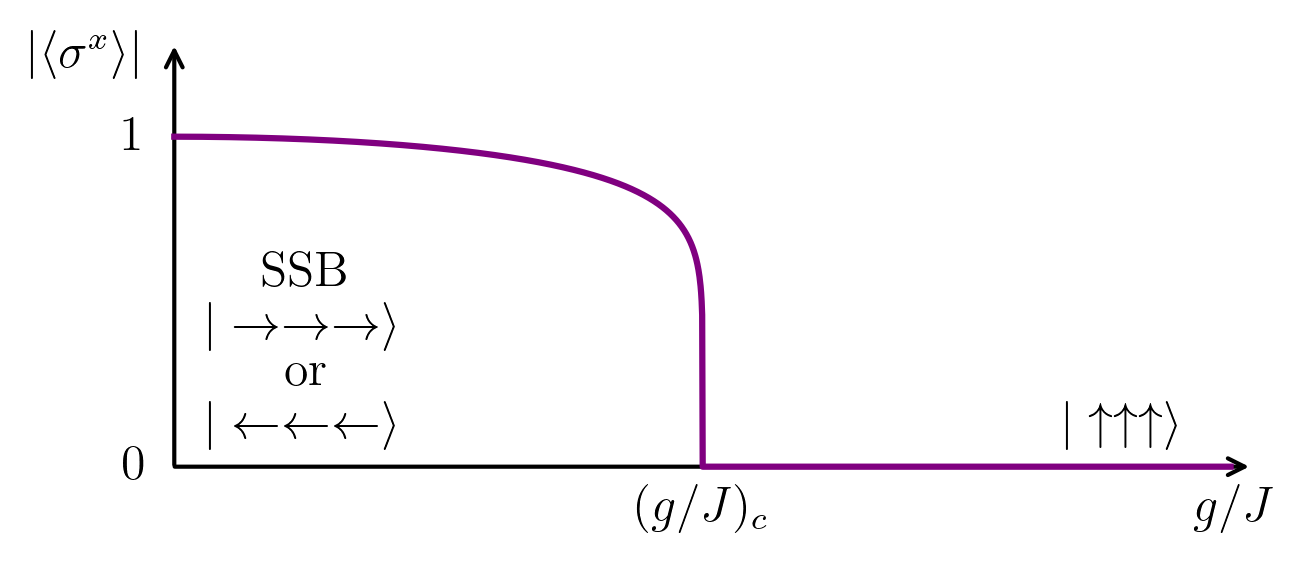
\includegraphics[width=0.7\linewidth]{tfi_phase_diagram.png}
  \caption{Qualitative quantum phase diagram for the TFI model on a hypercubic lattice. For $g \ll J$ the system spontaneously chooses one of the two degenerate, symmetry-broken ground states $\ket{\Rightarrow}$ and $\ket{\Leftarrow}$, with ferromagnetic magnetizations $\langle \sigma^x \rangle= 1$ and $\langle \sigma^x \rangle = -1$. With increasing $g/J$, quantum fluctuations reduce the magnetization magnitude to the value $0$ at the critical point, where the system undergoes a quantum phase transition to a paramagnetic phase with unique symmetric ground state ($\ket{\Uparrow}$ for $g \gg J$). Analytical solution and Monte Carlo simulations yield $g_c = J$ and $g_c \approx 3.044J$ in 1D and 2D, respectively.}
\label{fig:tfi_phase_diagram}
\end{figure}


% PERTURBATION THEORY
\section{Perturbation theory for large and small transverse field} \label{sec:tfi_perturbation_theory}

As a next step we want to find out how the degenerate first excited levels are quantitatively shifted when slightly moving away from the extreme limits $g \gg J$ and $g \ll J$. \\

\noindent Suppose we have a Hamiltonian $H^0$ which is easily diagonalized into degenerate groups (labelled by Greek letters) and orthonormal states within these groups (labelled by Latin letters): 
\begin{equation}
	H^0 \ket{\alpha, n} = E_{\alpha} \ket{\alpha, n}.
\end{equation}
We investigate the influence of a perturbation $\lambda V$, which is controlled by a small perturbation parameter $\lambda$. We assume that the energy differences $\vert E_{\alpha} - E_{\beta} \vert$ between groups are sufficiently large and use the effective Hamiltonian method \cite{sachdev2011quantum}, which unitarily eliminates nonzero inter-group matrix elements to restrict the study to modified energy levels within each group. Going from the unperturbed energies in zeroth order up to second order in perturbation theory, the effective intra-group matrix elements are given by
\begin{equation} \label{eq:H_eff}
	\bra{\alpha, n} H_{\text{eff}, \alpha} \ket{\alpha, m} = E_{\alpha} \delta_{n, m} + \lambda \bra{\alpha, n} V \ket{\alpha, m} + \lambda^2 \sum_{\beta \neq \alpha} \sum_{l} \frac{\bra{\alpha, n} V \ket{\beta, l} \bra{\beta, l} V \ket{\alpha, m}}{E_{\alpha} - E_{\beta}}.
\end{equation}
 The first order term accounts for the direct perturbation overlap between states within the same group. The second order term captures the indirect effect of states from other groups, via virtual transitions and back, weighted by the corresponding energy difference. \\
 
 \noindent For the TFI Hamiltonians $H(g \gg J)$ and $H(g \ll J)$ with periodic boundary conditions, we separate the single quasiparticle excitations $\{ \ket{n} \}$ from the vacuum ground state $\ket{0}$ below and the two particle states $\{ \ket{n, m} \}$ above. We then compute the effective Hamiltonians \eqref{eq:H_eff} for small perturbations $J V$ and $g V$, which all describe a single particle on a lattice with on-site energy $\mu$ and nearest-neighbor hopping $t$:
 \begin{equation}
 	H_{\text{eff}} =  
	 \mu \sum_n \vert n \rangle \langle n \vert 
	- t \sum_{\langle n, m \rangle} \left( \vert n \rangle \langle m \vert + \vert m \rangle \langle n \vert \right).
 \end{equation}
Diagonalization is easily achieved by Fourier transformation $\ket{n} = \frac{1}{\sqrt{N}} \sum_p e^{-ip \cdot n} \ket{p}$:
\begin{equation}
	H_{\text{eff}} = \sum_p \epsilon_p \ket{p}\bra{p},
\end{equation}
with $\epsilon_p =  \mu - 2t \cos(p)$ in one dimension and $\epsilon_p =  \mu - 2t \left[ \cos(p_x) + \cos(p_y) \right]$ in two dimensions. \\

\noindent In the following we denote with $\Delta_{\alpha} = E_{\alpha} - E_0$ the unperturbed energy of group $\alpha$ above the ground state. \\

\noindent $\underline{\underline{g \gg J}}$: $H^0 = - g \sum\limits_n \sigma^z_n$, $\lambda = J$, $V = - \sum\limits_{\langle n,m \rangle} \sigma^x_n \sigma^x_m$.
\begin{enumerate}
	\item[0)] Unique zero particle ground state $\ket{0} = \ket{\uparrow ... \uparrow}$,
	\item[1)] $N$ single particle states $\ket{n} =  \ket{\uparrow ... \uparrow \underset{\textcolor{blue}{n}}{\textcolor{blue}{\downarrow}} \uparrow ... \uparrow}$ with $\Delta_1 = 2g$,
	\item[2)] $N(N-1)/2$ two particle scattering states $\ket{n, m} = \ket{\uparrow ... \uparrow \underset{\textcolor{blue}{n}}{\textcolor{blue}{\downarrow}} \uparrow ... \uparrow \underset{\textcolor{blue}{m}}{\textcolor{blue}{\downarrow}} \uparrow ... \uparrow}$ with $\Delta_2 = 4g$.
\end{enumerate}
\noindent $\mathcal{O}(J)$: $J \bra{n} V \ket{m} = -J$ for $n, m$ nearest neighbors and $0$ else $\leadsto \mu = \Delta_1, t = J$. \\
\begin{equation} \label{eq:dispersion_large_g}
	\text{\underline{One dimension}}: \epsilon_p = 2g - 2J \cos(p) + \mathcal{O}(J^2),
\end{equation}
\begin{equation}
	\text{\underline{Two dimensions}}: \epsilon_p = 2g - 2J \left[\cos(p_x) + \cos(p_y)\right] + \mathcal{O}(J^2) . 
\end{equation}

\vspace*{1.5em}
\noindent $\underline{\underline{g \ll J}}$: $H^0 = -J \sum\limits_{\langle n,m \rangle} \sigma^x_n \sigma^x_m$, $\lambda = g$, $V = - \sum\limits_n \sigma^z_n$. \\

\noindent In this limit, qualitatively different lowest excitations emerge for the different spatial dimensions, so we treat them as separate cases. \\

\noindent \underline{One dimension}
\begin{enumerate}
	\item[0)] Zero particle ground state $\ket{0} = \ket{\rightarrow ... \rightarrow}$ or $\ket{0} = \ket{\leftarrow ... \leftarrow}$,
	\item[1)] $N$ single\footnote{Strictly speaking, for PBC domain walls always come in pairs. But they are really independent excitations and so we treat them as individually existing particles here.} domain wall states $\ket{n} =  \ket{\rightarrow ... \rightarrow \underset{\textcolor{blue}{n}}{}\textcolor{blue}{\leftarrow} \textcolor{blue}{ ... \leftarrow}}$ with $\Delta_1 = 2J$,
	\item[2)] $N(N-1)/2$ two domain wall scattering states $\ket{n, m} = \ket{\rightarrow ... \rightarrow \underset{\textcolor{blue}{n}}{} \textcolor{blue} {\leftarrow}\: \textcolor{blue}{ ... \leftarrow} \underset{\textcolor{blue}{m}}{} \rightarrow ... \rightarrow}$ with $\Delta_2 = 4J$.
\end{enumerate}
\noindent $\mathcal{O}(g)$: $g \bra{n} V \ket{m} = -g$ for $n, m$ nearest neighbors and $0$ else $\leadsto \mu = \Delta_1, t = g$. \\
\begin{equation} \label{eq:dispersion_small_g}
	\Rightarrow \epsilon_p = 2J - 2g \cos(p) + \mathcal{O}(g^2).
\end{equation}

\noindent \underline{Two dimensions}
\begin{enumerate}
	\item[0)] Zero particle ground state $\: \begin{matrix} \rightarrow & \rightarrow & \rightarrow & \rightarrow \\  \rightarrow & \rightarrow & \rightarrow & \rightarrow \\ \rightarrow & \rightarrow & \rightarrow & \rightarrow \\ \rightarrow & \rightarrow & \rightarrow & \rightarrow \\ \end{matrix} \:$ or $\: \begin{matrix} \leftarrow & \leftarrow & \leftarrow & \leftarrow \\  \leftarrow & \leftarrow & \leftarrow & \leftarrow \\ \leftarrow & \leftarrow & \leftarrow & \leftarrow \\ \leftarrow & \leftarrow & \leftarrow & \leftarrow \\ \end{matrix} \:$,
	\item[1)] $N$ single particle states $\: \begin{matrix} \rightarrow & \rightarrow & \rightarrow & \rightarrow \\  \rightarrow & \textcolor{blue}{\leftarrow} & \rightarrow & \rightarrow \\ \rightarrow & \rightarrow & \rightarrow & \rightarrow \\ \rightarrow & \rightarrow & \rightarrow & \rightarrow \\ \end{matrix} \:$ with $\Delta_1 = 8J$,
	\item[2)] $2N$ nearest-neighbor bound states $\: \begin{matrix} \rightarrow & \rightarrow & \rightarrow & \rightarrow \\  \rightarrow & \textcolor{blue}{\leftarrow} & \textcolor{blue}{\leftarrow} & \rightarrow \\ \rightarrow & \rightarrow & \rightarrow & \rightarrow \\ \rightarrow & \rightarrow & \rightarrow & \rightarrow \\ \end{matrix} \:$, $\: \begin{matrix} \rightarrow & \rightarrow & \rightarrow & \rightarrow \\  \rightarrow & \textcolor{blue}{\leftarrow} & \rightarrow & \rightarrow \\ \rightarrow & \textcolor{blue}{\leftarrow} & \rightarrow & \rightarrow \\ \rightarrow & \rightarrow & \rightarrow & \rightarrow \\ \end{matrix} \:$ with $\Delta_2 = 12J$,
	\item[3)] $N(N-1)/2 - 2N$ two particle scattering states $\: \begin{matrix} \rightarrow & \rightarrow & \rightarrow & \rightarrow \\ \rightarrow & \textcolor{blue}{\leftarrow} & \rightarrow & \rightarrow \\ \rightarrow & \rightarrow & \textcolor{blue}{\leftarrow} & \rightarrow \\ \rightarrow & \rightarrow & \rightarrow & \rightarrow \\ \end{matrix} \:$ with $\Delta_3 = 16J$.\footnote{The three particle bound states with energy $\Delta_4 = 14$ lie below the two particle scattering states. But since they have no overlap with the single particle states up to second order, we do not consider them here.}
\end{enumerate}
\noindent $\mathcal{O}(g)$: The perturbation $V$ brings the single particle states out of their degenerate subspace, so there is no nonzero matrix element in first order. \\

\noindent $\mathcal{O}(g^2)$: By drawing one representative of each (sub)group $\beta$ and multiplying with the number of equivalent states, we diagrammatically calculate the matrix elements 
\begin{equation}
\sum_{\beta=0),2),3)} \sum_{l} \frac{\bra{n} V \ket{\beta, l} \bra{\beta, l} V \ket{m}}{8J - E_{\beta}}.
\end{equation}

\begin{itemize}
\item $n = m$:
$\begin{matrix} 
	\\ 
	\begin{matrix} \rightarrow & \rightarrow & \rightarrow & \rightarrow \\  \rightarrow & \textcolor{blue}{\leftarrow} & \rightarrow & \rightarrow \\ \rightarrow & \rightarrow & \rightarrow & \rightarrow \\ \rightarrow & \rightarrow & \rightarrow & \rightarrow \\  \end{matrix} \\ 
	\text{energy 8J} \\
\end{matrix}$ 
$\begin{Bmatrix}  
	\begin{matrix} \rightarrow & \rightarrow & \rightarrow & \rightarrow \\  \rightarrow & \rightarrow & \rightarrow & \rightarrow \\ \rightarrow & \rightarrow & \rightarrow & \rightarrow \\ \rightarrow & \rightarrow & \rightarrow & \rightarrow \\ \end{matrix} \\ 
	\text{1 state, energy 0} \\ 
	\\ 
	\begin{matrix} \rightarrow & \rightarrow & \rightarrow & \rightarrow \\  \rightarrow & \textcolor{blue}{\leftarrow} & \textcolor{blue}{\leftarrow} & \rightarrow \\ \rightarrow & \rightarrow & \rightarrow & \rightarrow \\ \rightarrow & \rightarrow & \rightarrow & \rightarrow \\ \end{matrix} \\
	\text{4 states, energy 12J} \\ 
	\\ 
	\begin{matrix} \rightarrow & \rightarrow & \rightarrow & \rightarrow \\  \rightarrow & \textcolor{blue}{\leftarrow} & \rightarrow & \rightarrow \\ \rightarrow & \rightarrow & \textcolor{blue}{\leftarrow} & \rightarrow \\ \rightarrow & \rightarrow & \rightarrow & \rightarrow \\ \end{matrix} \\ 
	N\text{-5 states, energy 16J} \\
\end{Bmatrix}$
$\begin{matrix} 
	\\ 
	\begin{matrix} \rightarrow & \rightarrow & \rightarrow & \rightarrow \\  \rightarrow & \textcolor{blue}{\leftarrow} & \rightarrow & \rightarrow \\ \rightarrow & \rightarrow & \rightarrow & \rightarrow \\ \rightarrow & \rightarrow & \rightarrow & \rightarrow \\  \end{matrix} \\ 
	\text{energy 8J} \\
\end{matrix}$  
$\leadsto -\frac{N + 2}{8J} \ket{n}\bra{n}$, \\
	
\item $\vert n -m \vert = 1$:
$\begin{matrix}
	\\
	\begin{matrix} \rightarrow & \rightarrow & \rightarrow & \rightarrow \\  \rightarrow & \textcolor{blue}{\leftarrow} & \rightarrow & \rightarrow \\ \rightarrow & \rightarrow & \rightarrow & \rightarrow \\ \rightarrow & \rightarrow & \rightarrow & \rightarrow \\ \end{matrix} \\
	\text{energy 8J} \\
\end{matrix}$
$\begin{Bmatrix}
	\begin{matrix} \rightarrow & \rightarrow & \rightarrow & \rightarrow \\  \rightarrow & \rightarrow & \rightarrow & \rightarrow \\ \rightarrow & \rightarrow & \rightarrow & \rightarrow \\ \rightarrow & \rightarrow & \rightarrow & \rightarrow \\ \end{matrix} \\
	\text{1 state, energy 0} \\ 
	\\
	\begin{matrix} \rightarrow & \rightarrow & \rightarrow & \rightarrow \\  \rightarrow & \textcolor{blue}{\leftarrow} & \textcolor{blue}{\leftarrow} & \rightarrow \\ \rightarrow & \rightarrow & \rightarrow & \rightarrow \\ \rightarrow & \rightarrow & \rightarrow & \rightarrow \\ \end{matrix} \\
	\text{1 state, energy 12J} \\
\end{Bmatrix}$
$\begin{matrix}
	\\
	\begin{matrix} \rightarrow & \rightarrow & \rightarrow & \rightarrow \\  \rightarrow & \rightarrow & \textcolor{blue}{\leftarrow} & \rightarrow \\ \rightarrow & \rightarrow & \rightarrow & \rightarrow \\ \rightarrow & \rightarrow & \rightarrow & \rightarrow \\ \end{matrix} \\
	\text{energy 8J} \\
\end{matrix}$
$\leadsto - \frac{1}{8J} \ket{n}\bra{m}$, \\
	
\item $\vert n - m \vert > 1$: 
$\begin{matrix}
	\\
	\begin{matrix} \rightarrow & \rightarrow & \rightarrow & \rightarrow \\  \rightarrow & \textcolor{blue}{\leftarrow} & \rightarrow & \rightarrow \\ \rightarrow & \rightarrow & \rightarrow & \rightarrow \\ \rightarrow & \rightarrow & \rightarrow & \rightarrow \\ \end{matrix} \\
	\text{energy 8J} \\
\end{matrix}$
$\begin{Bmatrix}
	\begin{matrix} \rightarrow & \rightarrow & \rightarrow & \rightarrow \\  \rightarrow & \rightarrow & \rightarrow & \rightarrow \\ \rightarrow & \rightarrow & \rightarrow & \rightarrow \\ \rightarrow & \rightarrow & \rightarrow & \rightarrow \\ \end{matrix} \\
	\text{1 state, energy 0} \\ 
	\uparrow \\
	\text{cancel each other} \\
	\downarrow \\
	\begin{matrix} \rightarrow & \rightarrow & \rightarrow & \rightarrow \\  \rightarrow & \textcolor{blue}{\leftarrow} & \rightarrow & \rightarrow \\ \rightarrow & \rightarrow & \textcolor{blue}{\leftarrow} & \rightarrow \\ \rightarrow & \rightarrow & \rightarrow & \rightarrow \\ \end{matrix} \\
	\text{1 state, energy 16J} \\
\end{Bmatrix}$
$\begin{matrix}
	\\
	\begin{matrix} \rightarrow & \rightarrow & \rightarrow & \rightarrow \\  \rightarrow & \rightarrow & \rightarrow & \rightarrow \\ \rightarrow & \rightarrow & \textcolor{blue}{\leftarrow} & \rightarrow \\ \rightarrow & \rightarrow & \rightarrow & \rightarrow \\ \end{matrix} \\
	\text{energy 8J} \\
\end{matrix}$
$\leadsto 0$.
\end{itemize}

\noindent Note that in second order also the ground state energy is shifted.
\begin{itemize}
\item ground state:
$\begin{matrix} 
\begin{matrix} \rightarrow & \rightarrow & \rightarrow & \rightarrow \\  \rightarrow & \rightarrow & \rightarrow & \rightarrow \\ \rightarrow & \rightarrow & \rightarrow & \rightarrow \\ \rightarrow & \rightarrow & \rightarrow & \rightarrow \\ \end{matrix} \\
\text{energy 0} \\
\end{matrix}$
$\begin{Bmatrix}
\begin{matrix} \rightarrow & \rightarrow & \rightarrow & \rightarrow \\  \rightarrow & \textcolor{blue}{\leftarrow} & \rightarrow & \rightarrow \\ \rightarrow & \rightarrow & \rightarrow & \rightarrow \\ \rightarrow & \rightarrow & \rightarrow & \rightarrow \\ \end{matrix}  \\
N\text{ states, energy 8J} \\
\end{Bmatrix}$
$\begin{matrix}
\begin{matrix} \rightarrow & \rightarrow & \rightarrow & \rightarrow \\  \rightarrow & \rightarrow & \rightarrow & \rightarrow \\ \rightarrow & \rightarrow & \rightarrow & \rightarrow \\ \rightarrow & \rightarrow & \rightarrow & \rightarrow \\ \end{matrix} \\
\text{energy 0} \\
\end{matrix}$
$\leadsto - \frac{N}{8J}$. \\
\end{itemize}

\noindent $\leadsto$ We subtract $-N/(8J)$ as an energy offset and end up with $\mu = \Delta_1 - g^2/(4J)$, $t = g^2/(8J)$. \\
\begin{equation}
\Rightarrow \epsilon_p = 8J - \frac{g^2}{4J}[1 + \cos(p_x) + \cos(p_y)] + \mathcal{O}(g^3). 
\end{equation}

\vspace*{1em}
\noindent At this point a comment about the spontaneous symmetry breaking for $g \ll J$ is in order. If we pushed the perturbation theory up to $N$-th order for finite $N$, the degeneracy between the symmetric ground states $\frac{1}{\sqrt{2}} \left( \ket{\Rightarrow} \pm \ket{\Leftarrow} \right)$ would be lifted by an exponentially small energy splitting $\delta E_{\pm} = \mathcal{O}(g^N)$. SSB is thus restricted to the thermodynamic limit $N \to \infty$, where there is no tunneling matrix element between $\ket{\Rightarrow}$ and $\ket{\Leftarrow}$ at any finite order in $g$. We will see in section \ref{sec:dmrg} that DMRG is able to detect the energy splitting $\delta E_{\pm}$ for small enough $N$.


% EXACT SOLUTION
\section{Exact solution in one dimension} \label{sec:tfi_exact_solution}
\noindent In one dimension, the spectrum of the TFI model is exactly solvable for all values of $g$. The Hamiltonian \eqref{eq:tfi_hamiltonian} with periodic boundary conditions (PBC) $\sigma^x_{N+1} \equiv \sigma^x_1$ is
\begin{equation} \label{eq_ising_hamiltonian_1d}
	H = -J \sum_{n=1}^N \sigma^x_n \sigma^x_{n+1} - g \sum_{n=1}^N \sigma^z_n.
\end{equation}
We show the detailed calculations in appendix \ref{ch:detailed_tfi_solution}, and only summarize the three fundamental steps here \cite{pfeuty1970one, sachdev2011quantum}:
\begin{enumerate}
	\item[1)] \textit{Jordan-Wigner transformation}---Mapping spin-1/2 degrees of freedom to spinless fermions.
	\begin{equation}
		\sigma^z_n = 1 - 2c_n^{\dagger}c_n \:\: \text{and} \:\: \sigma^x_n = \eta_n (c_n^{\dagger} + c_n),
	\end{equation}
	where $\eta_n = \prod_{m<n}(1-2c_m^{\dagger}c_m)$ is the non-local Jordan-Wigner string. The Hamiltonian block diagonalizes into sectors of even/odd fermion parity,
\begin{equation}
	P_f = (-1)^{N_f} = (-1)^{\sum_n c_n^{\dagger} c_n} = \prod_n \sigma^z_n,
\end{equation}
when we impose anti-periodic boundary conditions $c_{N+1} = -c_1$ for $P_f = 1$ and periodic boundary conditions $c_{N+1} = c_1$ for $P_f = -1$.	
	\item[2)] \textit{Fourier transformation}---Going to momentum space.
	\begin{equation}
		c_n = \frac{1}{\sqrt{N}}\sum_p e^{-ipn}c_p,
	\end{equation}
	for momenta $p = \frac{2 \pi}{N}k$ with $k$ quantized to half-integers for $P_f = 1$ and to integers for $P_f = -1$.
	
	\item[3)] \textit{Bogoliubov transformation}---Diagonalizing the quadratic Hamiltonian.
	\begin{equation}
		\gamma_p = u_p c_p - i v_p c_{-p}^{\dagger},
	\end{equation}
	where $u_p = \cos(\frac{\vartheta_p}{2})$, $v_p = \sin(\frac{\vartheta_p}{2})$ and $\tan(\vartheta_p) = -\frac{J\sin(p)}{g - J\cos(p)}$. \\
\end{enumerate}

\noindent The final Hamiltonian in terms of fermionic creation and annihilation operators reads
\begin{equation}
	H = E_0 + \sum_p \epsilon_p \gamma_p^{\dagger} \gamma_p \:\:\: \text{with} \:\: \epsilon_p = 2\sqrt{g^2 - 2 J g \cos(p) + J^2}.
\end{equation}
The ground state with energy $E_0 = - \sum_p \epsilon_p/2$ is given by the vacuum $\ket{0}$ satisfying $\gamma_p \ket{0} = 0$ for all $p$. A single excitation with energy $\epsilon_p$ is created above by adding a fermion with corresponding momentum: $\ket{p} = \gamma_p^{\dagger} \ket{0}$. In a general $M$-particle state $\gamma_{p_1}^{\dagger} \cdots \gamma_{p_M}^{\dagger} \ket{0}$, the fermions occupy $M$ distinct single particle states and their total energy adds up to $\sum_{m=1}^M \epsilon_{p_m}$. \\

\noindent Note that the exact dispersion relation $\epsilon_p$ agrees with the perturbative ones for large \eqref{eq:dispersion_large_g} and small \eqref{eq:dispersion_small_g} $g/J$. For the transition between these limits, the exact solution adds a valuable insight. The energy gap $\epsilon_0$ closes at $g_c = J$, which quantitatively locates the critical point.